\documentclass{article}
\usepackage[a4paper, total={7.5in, 10in}]{geometry}
\geometry{paperwidth=10in, 
	%paperheight=16383pt, 
	paperheight=8100pt,
	left=2in, top=40pt, textwidth=6in, marginparsep=20pt, marginparwidth=1.5in, %textheight=16263pt, 
	textheight=8000pt,
	footskip=40pt
}
\usepackage{graphicx}
\usepackage{url}
\usepackage{natbib}
\usepackage{todonotes}
\usepackage{booktabs}
\usepackage{lineno}
\usepackage{color}
%\usepackage{auto-pst-pdf}
\usepackage[colaction]{multicol}
\usepackage{caption}
\usepackage{svg}
\usepackage{authblk}
\usepackage{standalone}
\usepackage[section]{placeins}


\linespread{1.5}

\makeatletter
\renewcommand{\maketitle}{\bgroup\setlength{\parindent}{0pt}
	\begin{flushleft}

		{\huge\textbf{\@title}}

		\bigskip

 		{\large\textbf{\@author}}

 		\bigskip

 		{\large{Draft current \@date}}

	\end{flushleft}\egroup
}
\makeatother

\newcommand{\multicollinenumbers}{
	\linenumbers
	\def\makeLineNumber{\docolaction
		{\makeLineNumberLeft}
		{}
		{\makeLineNumberRight}
		}
}

\newenvironment{figurehere}
	{\def\@captype{figure}}
	{}

% Title
\title{A Topic Model of Climate Change Literature}
\title{Words, words, words: Mapping the Matter of Climate Change Literature}
\title{A Topography of Climate Change Research - Results}
\author[1,2]{Max Callaghan}

\affil[1]{Mercator Research Institute on Global Commons and Climate Change, Torgauer Straße, 10829 Berlin, Germany}
\affil[2]{School of Earth and Environment, University of Leeds, Leeds LS2 9JT, United Kingdom}

\begin{document}
\maketitle

\section{Results}

\setcounter{totalnumber}{200}

\subsection{Literature growth}
	
\begin{table}[h]
	\scriptsize
	\begin{tabular}{|l |p{1.8cm} p{1.8cm} p{1.8cm} p{1.8cm} p{1.8cm} p{1.8cm}|} 
\hline 
&\textbf{AR1} & \textbf{AR2} & \textbf{AR3} & \textbf{AR4} & \textbf{AR5} & \textbf{AR6}\\ \hline\textbf{Years} &1986-1989 & 1990-1994 & 1995-2000 & 2001-2006 & 2007-2013 & 2014-\\ 
\textbf{Documents} &1,167 & 8,539 & 21,716 & 38,750 & 134,413 & 201,606\\ 
\textbf{Unique words} &2,000 & 12,480 & 23,346 & 34,637 & 71,867 & 94,746\\ 
\textbf{New words} & change (560) & oil (287) & downscaling (217) & sres (234) & biochar (1,791) & mmms (313)\\ & climate (428) & deltac (283) & degreesc (187) & petm (95) & redd (1,113) & cop21 (234)\\ & co2 (318) & whole (256) & ncep (130) & amf (88) & cmip5 (679) & c3n4 (214)\\ & climatic (289) & tax (254) & fco (107) & sf5cf3 (86) & cmip3 (587) & sdg (187)\\ & model (288) & landscape (249) & pfc (98) & clc (81) & mofs (299) & zika (182)\\ & atmospheric (281) & alternative (243) & otcs (98) & embankment (81) & sdm (297) & ndcs (168)\\ & effect (280) & availability (242) & dtr (95) & cwd (79) & mof (275) & indc (164)\\ & global (224) & life (239) & nee (89) & etm (75) & biochars (252) & indcs (134) \\ \hline
\end{tabular}

	\caption{Growth in climate change literature}
	\label{growthtable}
\end{table}

%\begin{figure}[h]
%	\begin{center}
%		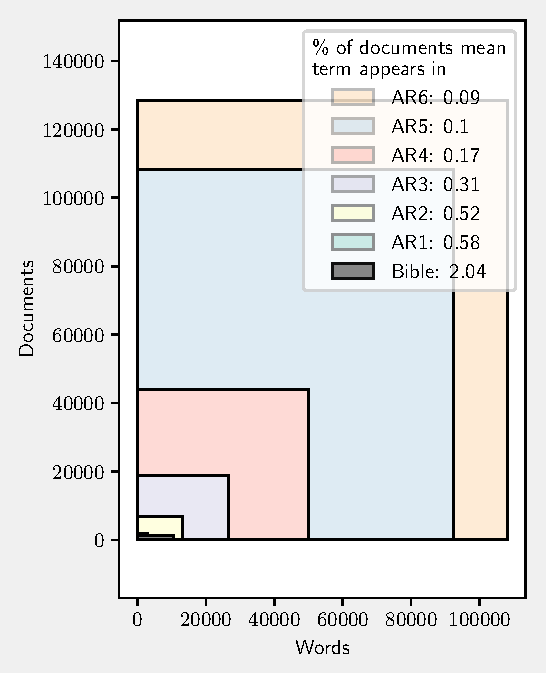
\includegraphics[width=0.5\linewidth]{plots/literature_size/volume_variety.pdf}
%		%\captionof{figure}
%		\caption{The volume and variety of literature on climate change has grown to unmanageable proportions. Each box represents a document-term matrix (unique documents x unique terms) of the abstracts written in each assessment period. The percentage of documents in which the average word occurs in is given in the key.
%		}
%	
%		\label{growth}
%	\end{center}
%\end{figure}



%\begin{figure}[h]
%	\begin{center}
%		%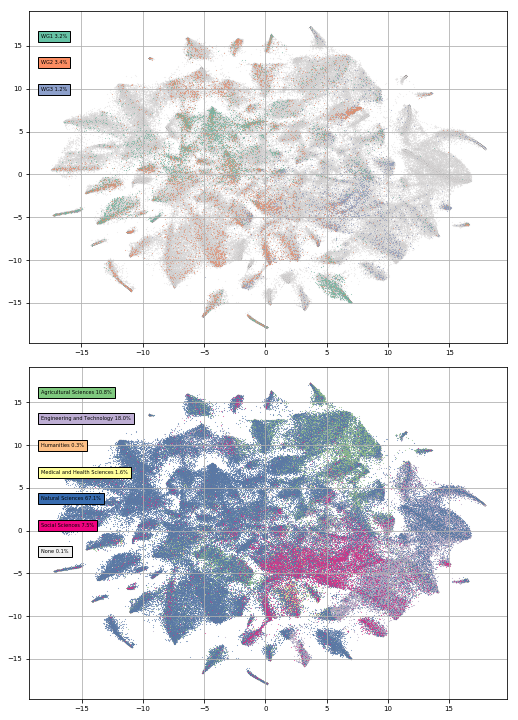
\includegraphics[width=1\linewidth]{tsne_results/plots/run_665_s_0_p200_double.pdf}
%		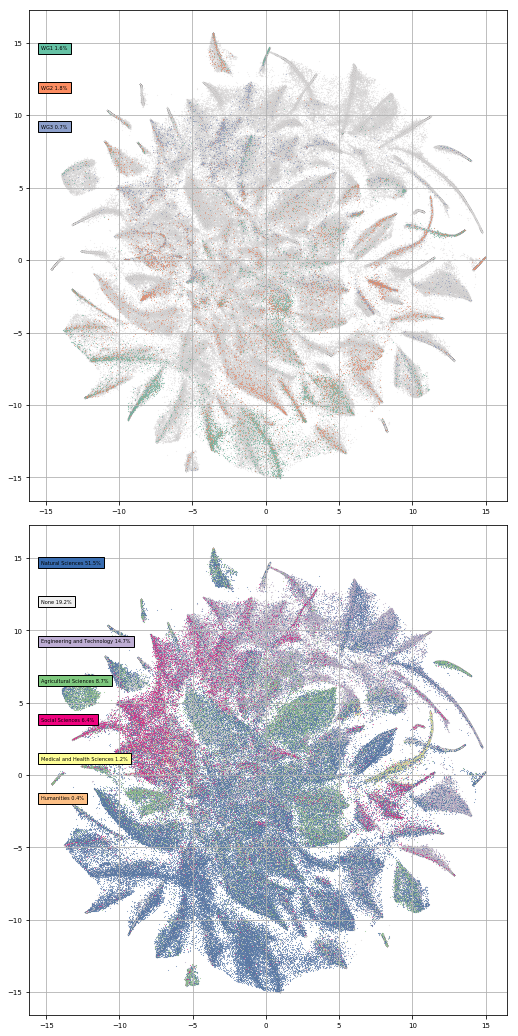
\includegraphics[width=0.85\linewidth]{tsne_results/plots/run_1275_s_0_p100_double.png}
%		\caption{A map of the literature on climate change. Document positions are obtained by reducing the topic scores to two dimensions via t-SNE Documents are coloured by working group citations (top) and web of science discipline category (bottom). See SI table for topic composition of each grid square}
%		\label{map-double}
%	\end{center}
%\end{figure}

\subsection{Disciplinary structure}

\todo{Label some topics particularly representative of certain disciplines, and their growth with reference to below}

\begin{figure}[h!]
	\begin{center}
		%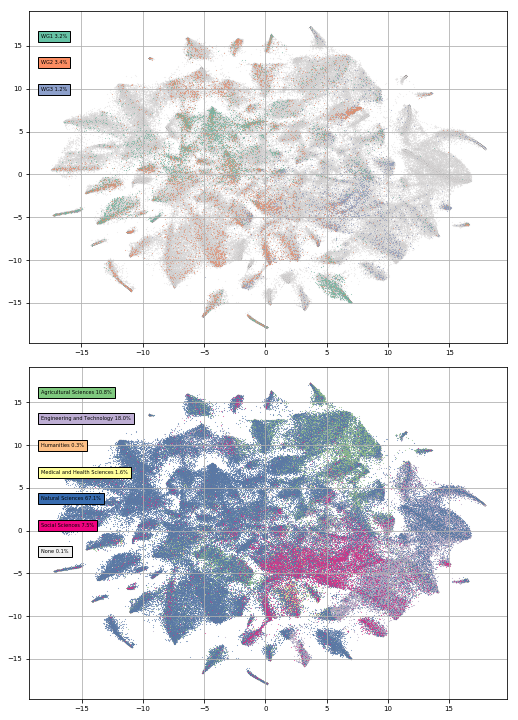
\includegraphics[width=1\linewidth]{tsne_results/plots/run_665_s_0_p200_double.pdf}
		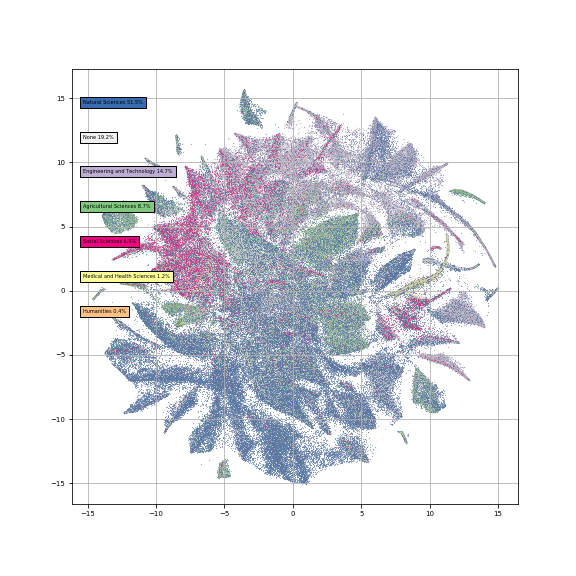
\includegraphics[width=1\linewidth]{tsne_results/plots/run_1275_s_0_p100_oecds.png}
		\caption{A map of the literature on climate change. Document positions are obtained by reducing the topic scores to two dimensions via t-SNE Documents are coloured by web of science discipline category. See SI table for topic composition of each grid square}
		\label{map-oecd}
	\end{center}
\end{figure}

\begin{itemize}
	\item The thematic structure of the topics reflects journal disciplinary categories. 
	\item Different disciplines clearly deal with different themes, although some topics are more interdisciplinary \todo{Show disciplinary entropy of topics in SI, give examples}
	\item Medicine has the most specialized topic distribution  
	\item (Some examples of individual topics using the labels to be added)
\end{itemize}

\bigskip

\begin{figure}[h!]
	\begin{center}
		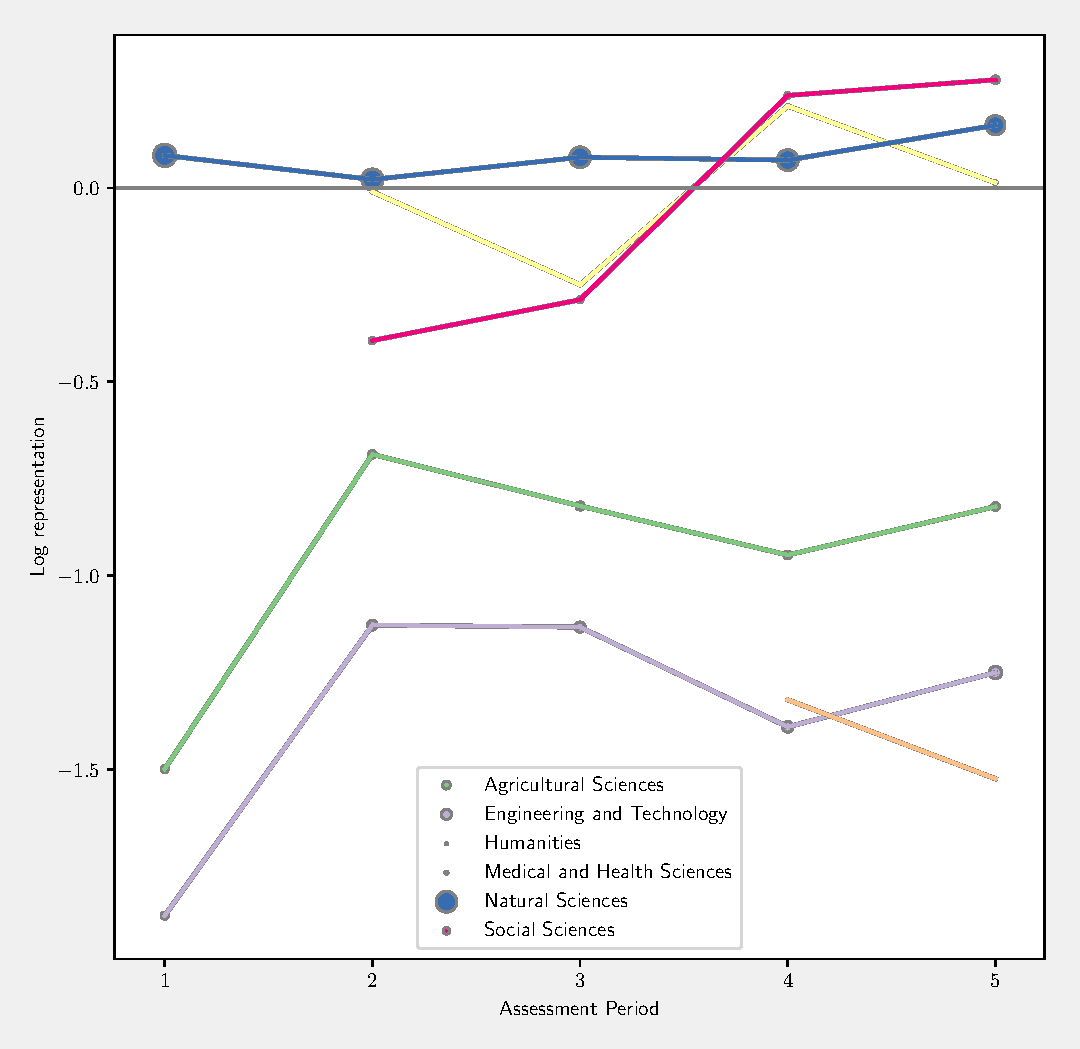
\includegraphics[width=0.85\linewidth]{plots/ipcc_representation/ipcc_rep_oecds_time.pdf}
		\caption{The representation within the IPCC of each discipline over time}
		\label{oecd_rep}
	\end{center}
\end{figure}

\begin{itemize}
	\item The natural sciences have always made up the greatest share of IPCC citations and documents about climate change
	\item The natural sciences were particularly over-represented in earlier assessment periods
	\item contrary to what is claimed, the natural sciences are not over-represented as compared to social sciences, these are now the most over-represented
	\item the disciplines that are under-represented are the agricultural sciences and engineering (also humanities to a small extent although they make up an extremely small share of all documents about climate change)
	\item (some examples of topics which portray this story - the ones which will be labelled above)
\end{itemize}

\bigskip

\subsection{IPCC working group structure}
\todo{Just 4 subplots, mashing together ar1-2, and 3-4}
\begin{figure}[h!]
	\begin{center}
		%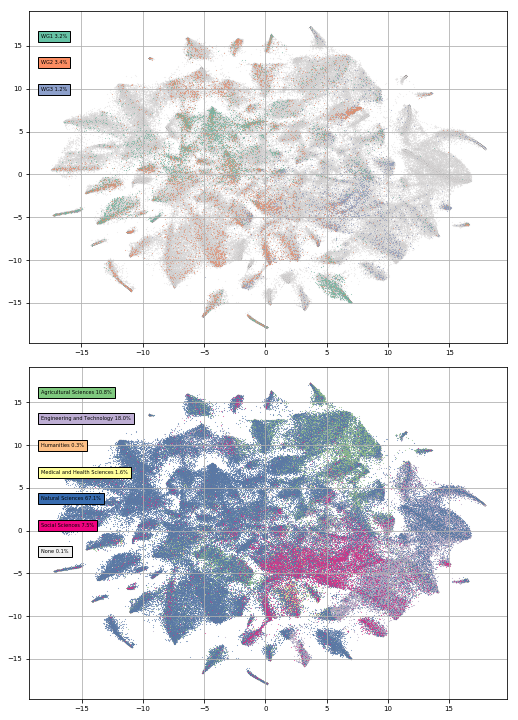
\includegraphics[width=1\linewidth]{tsne_results/plots/run_665_s_0_p200_double.pdf}
		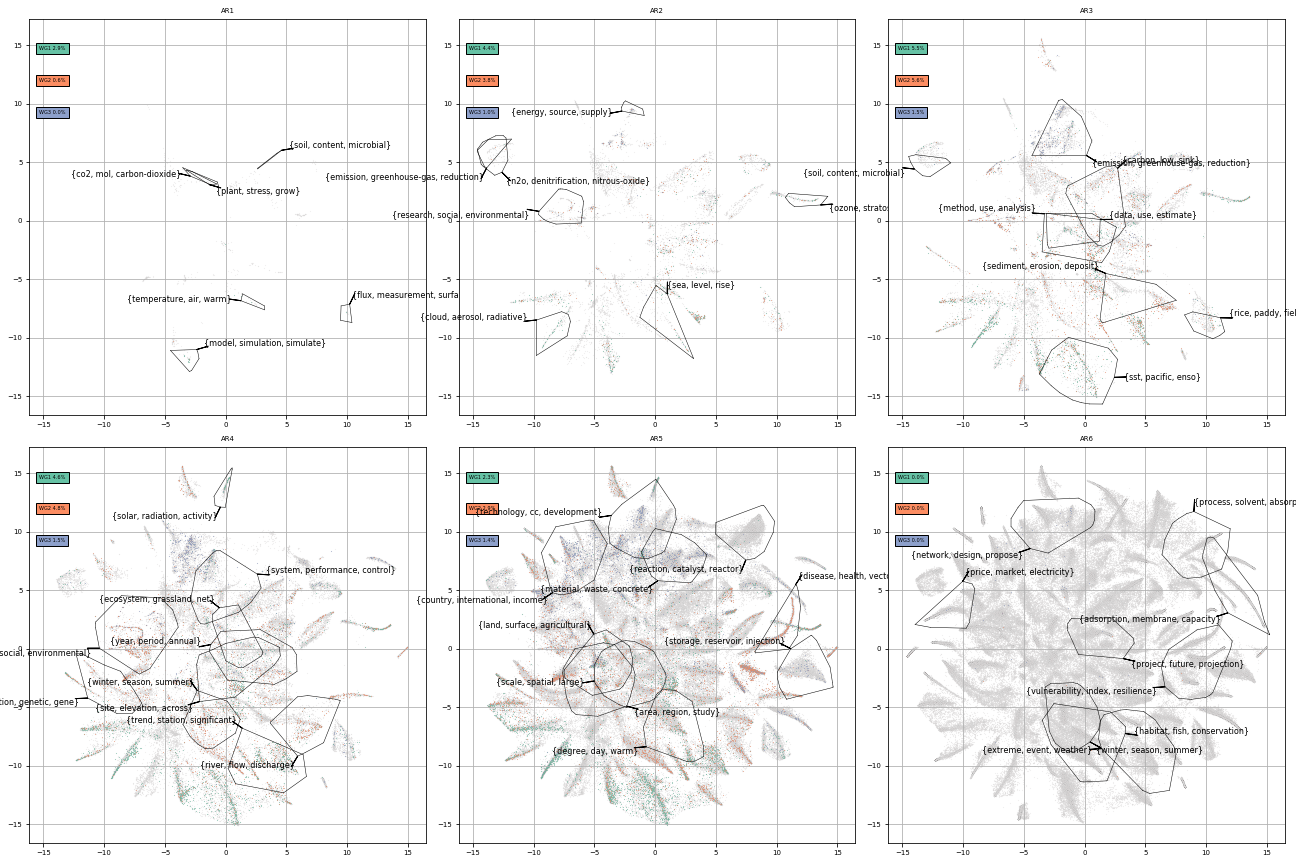
\includegraphics[width=1\linewidth]{tsne_results/plots/run_1275_s_0_p100_evolution.png}
		\caption{A map of the literature on climate change. Document positions are obtained by reducing the topic scores to two dimensions via t-SNE Documents are coloured by working group citations. In each assessment period, the largest cluster of documents relating to each of the 10 fastest growing topics is outlined.}
		\label{map-evolution}
		
	\end{center}
\end{figure}

\begin{itemize}
	\item The thematic structure is also reflected in the division of labour between IPCC working groups. Documents cited by each working group appear in discrete parts of the map (which correspond also to the disciplinary structure)
	\item Some topics cut across working groups [e.g. Urban, say more about]
	\item Some fast growing topics [e.g. health] are well represented in IPCC [WGII], whereas others (particularly on negative emissions) are not so well represented.
	
\end{itemize}

\begin{figure}[h!]
	\begin{center}
		\includegraphics[width=0.85\linewidth]{example-image}
		\caption{Optional figure, instead of above, one large wg map, with the topics below labelled}
		\label{ipcc_rep}
	\end{center}
\end{figure}

\begin{figure}[h!]
	\begin{center}
		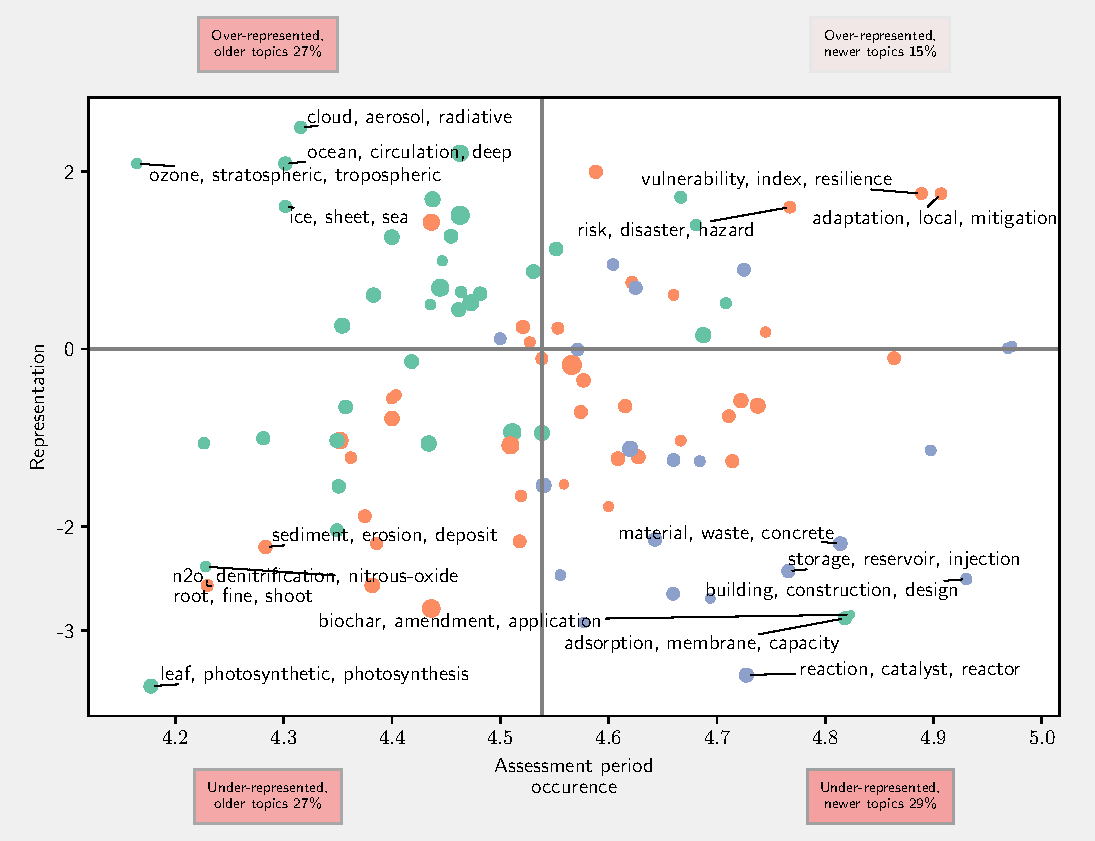
\includegraphics[width=0.85\linewidth]{plots/ipcc_representation/ipcc_rep_new1275_all.pdf}
		\caption{The IPCC representation and age of the topics. Representation shows the log of the share of topic documents in IPCC citations divided by the share of topic documents among all documents. Assessment period occurence shows the assessment period in which the mean topic document was published}
		\label{ipcc_rep}
	\end{center}
\end{figure}

\begin{itemize}
	\item Those topics that deal with working group III issues (materials and recycling, negative emissions, buildings) are in general fast growing and under-represented in IPCC reports
	\item Some working group III topics (on scenarios, on policies, and on international trade and cross country comparisons) are however over-represented in IPCC reports [see SI]
	\item Working group I topics are in general older and better represented. Could also be same topics but new knowledge
	\item Of the newer topics that are well represented, many are on WG III issues [detail required]
	\item Are WGII better at reflecting changes in the literature?
	\item Another plot showing lines for each topic showing growth in literature and growth in ipcc?
\end{itemize}

\section{SI}

\subsection{Glossary}

ncep
fco
pfc
otcs
dtr
sres
petm
amf
sf5cf3
clc
cwd
etm
cmip5
cmip3
mofs
sdm
mmms
cop21
c3n4
sdg
indc

\begin{table}[h!]
	\scriptsize
	\begin{tabular}{lrrrrlr}
\toprule
{} &  ipcc\_share &     share &  representation &  primary\_wg &                                   title &   year\_av \\
\midrule
0   &    0.006262 &  0.006395 &        0.979211 &           3 &       \{ghg, greenhouse-gas, mitigation\} &  4.780488 \\
1   &    0.000650 &  0.002675 &        0.243124 &           3 &       \{biochar, amendment, application\} &  4.758621 \\
2   &    0.002171 &  0.005588 &        0.388425 &           3 &         \{storage, reservoir, injection\} &  4.652174 \\
3   &    0.001689 &  0.005016 &        0.336741 &           3 &                  \{oil, palm, biodiesel\} &  4.644444 \\
4   &    0.001909 &  0.004702 &        0.406082 &           3 &       \{electricity, generation, demand\} &  4.634146 \\
5   &    0.009932 &  0.007924 &        1.253431 &           3 &             \{policy, government, maker\} &  4.634146 \\
6   &    0.001355 &  0.005430 &        0.249488 &           3 &            \{power, generation, nuclear\} &  4.627907 \\
7   &    0.000772 &  0.003433 &        0.224982 &           3 &            \{vehicle, electric, battery\} &  4.625000 \\
8   &    0.004662 &  0.007966 &        0.585245 &           3 &           \{technology, cc, development\} &  4.617021 \\
9   &    0.001251 &  0.005314 &        0.235373 &           3 &            \{cement, material, concrete\} &  4.615385 \\
10  &    0.004078 &  0.008273 &        0.492982 &           3 &                \{energy, demand, source\} &  4.595238 \\
11  &    0.006233 &  0.006769 &        0.920846 &           3 &                    \{price, market, tax\} &  4.577778 \\
12  &    0.004963 &  0.005667 &        0.875751 &           3 &          \{sector, industry, industrial\} &  4.571429 \\
13  &    0.001154 &  0.003121 &        0.369613 &           3 &                      \{soc, stock, soil\} &  4.568182 \\
14  &    0.000780 &  0.003826 &        0.203874 &           3 &                \{waste, landfill, solid\} &  4.568182 \\
15  &    0.005659 &  0.005908 &        0.957905 &           3 &              \{cost, benefit, abatement\} &  4.568182 \\
16  &    0.000812 &  0.003718 &        0.218338 &           3 &                \{coal, combustion, mine\} &  4.562500 \\
17  &    0.011040 &  0.008608 &        1.282596 &           3 &       \{country, develop, international\} &  4.543478 \\
18  &    0.010841 &  0.010172 &        1.065744 &           3 &             \{reduction, reduce, target\} &  4.533333 \\
19  &    0.002695 &  0.005586 &        0.482466 &           3 &                  \{fuel, fossil, engine\} &  4.500000 \\
20  &    0.048400 &  0.043462 &        1.113604 &           3 &   \{emission, greenhouse-gas, inventory\} &  4.500000 \\
21  &    0.011413 &  0.005391 &        2.117184 &           2 &   \{adaptation, vulnerability, strategy\} &  4.783784 \\
22  &    0.003123 &  0.004452 &        0.701476 &           2 &             \{urban, city, urbanization\} &  4.757576 \\
23  &    0.001268 &  0.004327 &        0.292959 &           2 &        \{building, construction, design\} &  4.702703 \\
24  &    0.006544 &  0.005171 &        1.265452 &           2 &                \{risk, disaster, hazard\} &  4.684211 \\
25  &    0.000978 &  0.004770 &        0.205070 &           2 &       \{adsorption, capacity, adsorbent\} &  4.676471 \\
26  &    0.003577 &  0.004542 &        0.787517 &           2 &        \{household, income, consumption\} &  4.676471 \\
27  &    0.005267 &  0.008168 &        0.644840 &           2 &   \{habitat, conservation, biodiversity\} &  4.674419 \\
28  &    0.003701 &  0.004579 &        0.808288 &           2 &                     \{food, web, supply\} &  4.650000 \\
29  &    0.003152 &  0.002859 &        1.102456 &           2 &                \{coral, reef, bleaching\} &  4.645833 \\
30  &    0.005709 &  0.005180 &        1.102186 &           2 &             \{health, public, mortality\} &  4.634146 \\
31  &    0.005419 &  0.007802 &        0.694545 &           2 &        \{management, resource, practice\} &  4.634146 \\
32  &    0.008456 &  0.011061 &        0.764468 &           2 &              \{research, science, issue\} &  4.634146 \\
33  &    0.006236 &  0.007047 &        0.884940 &           2 &        \{economic, development, economy\} &  4.625000 \\
34  &    0.004594 &  0.006687 &        0.687020 &           2 &            \{population, size, survival\} &  4.622222 \\
35  &    0.001609 &  0.005459 &        0.294757 &           2 &              \{genetic, diversity, gene\} &  4.619048 \\
36  &    0.004486 &  0.010488 &        0.427700 &           2 &              \{network, design, problem\} &  4.615385 \\
37  &    0.004747 &  0.005479 &        0.866385 &           2 &                 \{fish, fishery, marine\} &  4.613636 \\
38  &    0.007463 &  0.011144 &        0.669715 &           2 &           \{environmental, impact, life\} &  4.609756 \\
39  &    0.002422 &  0.004786 &        0.506071 &           2 &                    \{farm, animal, milk\} &  4.609756 \\
40  &    0.004245 &  0.006343 &        0.669241 &           2 &     \{community, microbial, composition\} &  4.609756 \\
41  &    0.004632 &  0.004635 &        0.999354 &           2 &                 \{disease, vector, host\} &  4.595745 \\
42  &    0.013609 &  0.009337 &        1.457572 &           2 &              \{project, cdm, projection\} &  4.595745 \\
43  &    0.003979 &  0.004463 &        0.891546 &           2 &             \{drought, severe, severity\} &  4.589744 \\
44  &    0.005927 &  0.008607 &        0.688619 &           2 &              \{specie, native, invasive\} &  4.586957 \\
45  &    0.001539 &  0.003043 &        0.505532 &           2 &        \{groundwater, recharge, aquifer\} &  4.581395 \\
46  &    0.002316 &  0.005242 &        0.441717 &           2 &       \{landscape, erosion, disturbance\} &  4.577778 \\
47  &    0.003614 &  0.003665 &        0.986025 &           2 &               \{flood, flooding, damage\} &  4.575000 \\
48  &    0.005727 &  0.008737 &        0.655430 &           2 &           \{system, performance, hybrid\} &  4.568182 \\
49  &    0.014225 &  0.006807 &        2.089702 &           2 &              \{scenario, future, impact\} &  4.568182 \\
50  &    0.005689 &  0.009700 &        0.586482 &           2 &               \{process, chemical, base\} &  4.568182 \\
51  &    0.007445 &  0.007451 &        0.999162 &           2 &              \{human, activity, natural\} &  4.555556 \\
52  &    0.004140 &  0.006229 &        0.664684 &           2 &                     \{flow, stream, low\} &  4.555556 \\
53  &    0.005146 &  0.005176 &        0.994293 &           2 &        \{crop, agricultural, irrigation\} &  4.547619 \\
54  &    0.008942 &  0.006187 &        1.445342 &           2 &               \{extreme, event, weather\} &  4.534884 \\
55  &    0.016558 &  0.017701 &        0.935400 &           2 &     \{index, vulnerability, correlation\} &  4.523810 \\
56  &    0.007844 &  0.007612 &        1.030470 &           2 &                \{stress, response, gene\} &  4.511628 \\
57  &    0.009577 &  0.012434 &        0.770286 &           2 &                     \{area, study, high\} &  4.511111 \\
58  &    0.003715 &  0.004875 &        0.761937 &           2 &               \{river, discharge, basin\} &  4.510638 \\
59  &    0.007486 &  0.007414 &        1.009739 &           2 &          \{ecosystem, net, productivity\} &  4.510638 \\
60  &    0.003211 &  0.003116 &        1.030511 &           2 &                  \{fire, burn, wildfire\} &  4.510204 \\
61  &    0.005322 &  0.005042 &        1.055661 &           2 &              \{runoff, catchment, basin\} &  4.489362 \\
62  &    0.007941 &  0.008078 &        0.982939 &           2 &            \{distribution, range, niche\} &  4.479167 \\
63  &    0.005792 &  0.008245 &        0.702468 &           2 &          \{production, primary, produce\} &  4.478261 \\
64  &    0.002472 &  0.003512 &        0.703775 &           2 &               \{wetland, coastal, marsh\} &  4.468085 \\
65  &    0.006171 &  0.004839 &        1.275431 &           2 &               \{rainfall, monsoon, rain\} &  4.458333 \\
66  &    0.011976 &  0.011338 &        1.056311 &           2 &           \{effect, affect, interaction\} &  4.456522 \\
67  &    0.007983 &  0.010211 &        0.781808 &           2 &           \{water, irrigation, resource\} &  4.456522 \\
68  &    0.011411 &  0.008555 &        1.333875 &           2 &               \{region, regional, south\} &  4.446809 \\
69  &    0.051512 &  0.035918 &        1.434134 &           2 &               \{increase, decrease, due\} &  4.428571 \\
70  &    0.003390 &  0.005339 &        0.634989 &           2 &       \{biomass, aboveground, bioenergy\} &  4.428571 \\
71  &    0.006279 &  0.006987 &        0.898570 &           2 &                   \{yield, wheat, grain\} &  4.428571 \\
72  &    0.012344 &  0.011019 &        1.120252 &           2 &                     \{term, long, short\} &  4.420000 \\
73  &    0.008298 &  0.009014 &        0.920592 &           2 &                     \{season, day, grow\} &  4.420000 \\
74  &    0.003944 &  0.007142 &        0.552150 &           2 &               \{site, elevation, across\} &  4.411765 \\
75  &    0.002282 &  0.004669 &        0.488863 &           2 &      \{litter, decomposition, microbial\} &  4.408163 \\
76  &    0.003608 &  0.005734 &        0.629128 &           2 &                     \{tree, ring, stand\} &  4.408163 \\
77  &    0.006229 &  0.006779 &        0.918986 &           2 &               \{forest, stand, tropical\} &  4.408163 \\
78  &    0.003427 &  0.007046 &        0.486287 &           2 &                     \{plant, seed, grow\} &  4.400000 \\
79  &    0.003690 &  0.006855 &        0.538355 &           2 &         \{nitrogen, nutrient, treatment\} &  4.395833 \\
80  &    0.019507 &  0.010818 &        1.803093 &           2 &               \{change, climatic, shift\} &  4.384615 \\
81  &    0.006852 &  0.007898 &        0.867560 &           2 &              \{rate, high, accumulation\} &  4.380000 \\
82  &    0.004288 &  0.006107 &        0.702157 &           2 &                  \{growth, radial, grow\} &  4.375000 \\
83  &    0.006251 &  0.012730 &        0.491062 &           2 &               \{soil, moisture, content\} &  4.372549 \\
84  &    0.006042 &  0.006238 &        0.968498 &           2 &               \{vegetation, ndvi, cover\} &  4.372549 \\
85  &    0.002689 &  0.005191 &        0.517979 &           2 &                   \{lake, level, diatom\} &  4.358491 \\
86  &    0.002031 &  0.005811 &        0.349411 &           2 &               \{sediment, erosion, core\} &  4.358491 \\
87  &    0.002397 &  0.003938 &        0.608762 &           2 &                    \{rice, paddy, field\} &  4.355556 \\
88  &    0.001554 &  0.004251 &        0.365605 &           2 &                     \{root, fine, shoot\} &  4.264151 \\
89  &    0.001861 &  0.004536 &        0.410171 &           2 &  \{leaf, photosynthesis, photosynthetic\} &  4.142857 \\
90  &    0.002603 &  0.005355 &        0.485996 &           1 &              \{china, province, chinese\} &  4.729730 \\
91  &    0.000328 &  0.003832 &        0.085614 &           1 &     \{membrane, separation, selectivity\} &  4.666667 \\
92  &    0.001056 &  0.004985 &        0.211908 &           1 &            \{absorption, solvent, amine\} &  4.634146 \\
93  &    0.001588 &  0.008110 &        0.195837 &           1 &             \{oxygen, reaction, reactor\} &  4.604651 \\
94  &    0.000631 &  0.004474 &        0.140983 &           1 &                 \{hydrogen, cell, steam\} &  4.571429 \\
95  &    0.012275 &  0.006043 &        2.031420 &           1 &      \{uncertainty, estimate, parameter\} &  4.565217 \\
96  &    0.007506 &  0.012308 &        0.609808 &           1 &                 \{method, use, approach\} &  4.558140 \\
97  &    0.004420 &  0.005373 &        0.822605 &           1 &                   \{heat, heating, pump\} &  4.547619 \\
98  &    0.004159 &  0.004082 &        1.019032 &           1 &                  \{wind, speed, turbine\} &  4.520833 \\
99  &    0.012651 &  0.007437 &        1.701127 &           1 &           \{trend, station, significant\} &  4.520833 \\
100 &    0.007889 &  0.005987 &        1.317745 &           1 &                  \{wave, coastal, storm\} &  4.511111 \\
101 &    0.014942 &  0.012453 &        1.199858 &           1 &                 \{scale, spatial, large\} &  4.510638 \\
102 &    0.008368 &  0.006040 &        1.385324 &           1 &             \{land, cover, agricultural\} &  4.500000 \\
103 &    0.009347 &  0.009705 &        0.963106 &           1 &                     \{carbon, low, sink\} &  4.468085 \\
104 &    0.008119 &  0.004261 &        1.905300 &           1 &              \{arctic, permafrost, warm\} &  4.448980 \\
105 &    0.009826 &  0.006145 &        1.598856 &           1 &       \{precipitation, annual, moisture\} &  4.446809 \\
106 &    0.007645 &  0.009833 &        0.777451 &           1 &                  \{data, use, satellite\} &  4.446809 \\
107 &    0.007591 &  0.006672 &        1.137725 &           1 &                 \{degree, day, latitude\} &  4.434783 \\
108 &    0.022381 &  0.009859 &        2.270102 &           1 &                 \{climate, future, warm\} &  4.431373 \\
109 &    0.021865 &  0.012745 &        1.715519 &           1 &           \{model, simulation, simulate\} &  4.428571 \\
110 &    0.003086 &  0.006655 &        0.463646 &           1 &                 \{gas, natural, hydrate\} &  4.428571 \\
111 &    0.002026 &  0.005943 &        0.340879 &           1 &              \{carbonate, mineral, rock\} &  4.420000 \\
112 &    0.013955 &  0.009888 &        1.411387 &           1 &               \{temperature, warm, mean\} &  4.420000 \\
113 &    0.004515 &  0.005048 &        0.894359 &           1 &       \{transport, road, transportation\} &  4.416667 \\
114 &    0.012788 &  0.008996 &        1.421430 &           1 &                \{winter, summer, spring\} &  4.415094 \\
115 &    0.013202 &  0.007618 &        1.733013 &           1 &                      \{sea, level, rise\} &  4.411765 \\
116 &    0.006158 &  0.006395 &        0.962925 &           1 &               \{air, pollution, quality\} &  4.408163 \\
117 &    0.004523 &  0.003533 &        1.280060 &           1 &                    \{snow, cover, depth\} &  4.400000 \\
118 &    0.008692 &  0.007754 &        1.121041 &           1 &                   \{per, thousand, part\} &  4.384615 \\
119 &    0.002843 &  0.006255 &        0.454437 &           1 &                 \{cal, pollen, holocene\} &  4.379310 \\
120 &    0.012002 &  0.009752 &        1.230792 &           1 &                  \{year, period, annual\} &  4.377358 \\
121 &    0.004178 &  0.003051 &        1.369399 &           1 &                \{glacier, mass, balance\} &  4.372549 \\
122 &    0.004935 &  0.004158 &        1.186828 &           1 &          \{solar, radiation, irradiance\} &  4.372549 \\
123 &    0.012949 &  0.005949 &        2.176902 &           1 &                    \{pacific, sst, enso\} &  4.351852 \\
124 &    0.025289 &  0.011214 &        2.255153 &           1 &                  \{global, earth, world\} &  4.346154 \\
125 &    0.015417 &  0.004451 &        3.463820 &           1 &           \{aerosol, forcing, radiative\} &  4.345455 \\
126 &    0.002264 &  0.004672 &        0.484521 &           1 &                 \{delta, isotope, value\} &  4.339286 \\
127 &    0.009276 &  0.010024 &        0.925337 &           1 &                   \{record, late, early\} &  4.298246 \\
128 &    0.014874 &  0.009238 &        1.610133 &           1 &                \{surface, layer, albedo\} &  4.296296 \\
129 &    0.007488 &  0.009212 &        0.812887 &           1 &              \{co2, mol, carbon-dioxide\} &  4.294118 \\
130 &    0.008833 &  0.007248 &        1.218694 &           1 &           \{glacial, last, interglacial\} &  4.271186 \\
131 &    0.011542 &  0.009860 &        1.170620 &           1 &              \{concentration, doc, high\} &  4.264151 \\
132 &    0.016337 &  0.006185 &        2.641400 &           1 &              \{ocean, circulation, deep\} &  4.258621 \\
133 &    0.005594 &  0.005752 &        0.972513 &           1 &                \{flux, measurement, net\} &  4.258621 \\
134 &    0.001581 &  0.003654 &        0.432735 &           1 &   \{n2o, denitrification, nitrous-oxide\} &  4.254902 \\
135 &    0.007908 &  0.003266 &        2.420887 &           1 &            \{cloud, feedback, radiative\} &  4.254545 \\
136 &    0.010994 &  0.005111 &        2.151092 &           1 &                       \{ice, sheet, sea\} &  4.229508 \\
137 &    0.003641 &  0.004293 &        0.848013 &           1 &            \{methane, oxidation, source\} &  4.218182 \\
138 &    0.002656 &  0.003766 &        0.705170 &           1 &                  \{ch4, oxidation, peat\} &  4.208333 \\
139 &    0.010688 &  0.003800 &        2.812635 &           1 &    \{ozone, stratospheric, tropospheric\} &  4.203390 \\
\bottomrule
\end{tabular}

	\caption{Top 10 topics in climate change literature}
	\label{top-topics}
\end{table}	

\begin{table}[h!]
	\scriptsize
	\begin{tabular}{p{1.9cm} p{3cm} p{7.5cm} r}
\toprule
                      title &                                                                            top words &                                                                                                                                                                                                                                                                top docs &   share \\
\midrule
      climat, chang, impact &          [climat, chang, impact, respons, futur, effect, shift, sensit, affect, may] &                                                                                                                                                  \parbox[t]{7.5cm}{Climate oscillations and changes over Russia; \\World Regionalization of Climate Change (1961-2010)} &  2.73\% \\
     soil, moistur, microbi &       [soil, moistur, microbi, organ, respir, content, miner, depth, matter, efflux] &                                                                                    \parbox[t]{7.5cm}{PARTITIONING OF SOIL RESPIRATION IN A FIRST ROTATION BEECH PLANTATION; \\Responses of soil respiration to N fertilization in a loamy soil under maize cultivation} &  2.73\% \\
       emiss, reduct, reduc &      [emiss, reduct, reduc, greenhous, factor, total, estim, inventori, nox, measur] &                                                                                                             \parbox[t]{7.5cm}{China's CH4 and CO2 emissions: Bottom-up estimation and comparative analysis; \\Monitoring total emissions from industrial installations} &  2.21\% \\
   carbon, dioxid, sequestr &   [carbon, dioxid, sequestr, sink, organ, cycl, storag, stock, terrestri, atmospher] &                             \parbox[t]{7.5cm}{Interpreting carbon-isotope excursions: carbonates and organic matter; \\PARTICULATE FLUXES OF CARBONATE AND ORGANIC-CARBON IN THE OCEAN - IS THE MARINE BIOLOGICAL-ACTIVITY WORKING AS A SINK OF THE ATMOSPHERIC CARBON} &  1.74\% \\
      temperatur, air, mean &  [temperatur, air, mean, surfac, minimum, maximum, daili, increas, effect, degreesc] &                                                                                                     \parbox[t]{7.5cm}{Observed changes in shallow soil temperatures in Northeast China, 1960-2007; \\Beyond the Mean: Biological Impacts of Cryptic Temperature Change} &  1.71\% \\
      record, dure, glacial &       [record, dure, glacial, reconstruct, last, period, holocen, event, late, core] &                                                           \parbox[t]{7.5cm}{HIGH-RESOLUTION CLIMATE RECORDS FROM THE NORTH-ATLANTIC DURING THE LAST INTERGLACIAL; \\HIGH-RESOLUTION CLIMATIC INFORMATION FROM SHORT FIRN CORES, WESTERN DRONNING MAUD LAND, ANTARCTICA} &   1.7\% \\
     speci, distribut, rang &          [speci, distribut, rang, rich, invas, nich, predict, extinct, shift, abund] &                               \parbox[t]{7.5cm}{Northward range extensions of some mesopelagic fishes in the Northeastern Atlantic; \\Natural occurrence and backwater infection of C-4 plants in the vegetation of the Yangtze hydropower Three Gorges Project region} &   1.7\% \\
 increas, concentr, decreas &   [increas, concentr, decreas, effect, atmospher, doc, result, organ, nutrient, may] &                                                          \parbox[t]{7.5cm}{TERRESTRIAL HIGHER-PLANT RESPONSE TO INCREASING ATMOSPHERIC [CO2] IN RELATION TO THE GLOBAL CARBON-CYCLE; \\Hydrological response to climate change in the Black Hills of South Dakota, USA} &  1.61\% \\
      forest, tropic, stand &       [forest, tropic, stand, deforest, disturb, stock, boreal, redd, harvest, wood] &  \parbox[t]{7.5cm}{Spatially explicit estimates and temporal changes of forest tree biomass in a typical department of forest management, Turkey; \\Analysis of the changes in forest ecosystem functions, structure and composition in the Black Sea region of Turkey} &  1.56\% \\
    energi, renew, consumpt &        [energi, renew, consumpt, effici, demand, save, sector, sourc, industri, use] &                                                                                                                                       \parbox[t]{7.5cm}{Energy issues and energy priorities; \\Energy efficiency and CO2 emissions in Swedish manufacturing industries} &  1.56\% \\
\bottomrule
\end{tabular}

	\caption{Top 10 topics in climate change literature}
	\label{top-topics}
\end{table}	

\end{document}